\documentclass[journal]{IEEEtran}
\usepackage{amsmath,amsfonts}
\usepackage{algorithmic}
\usepackage{algorithm}
\usepackage{array}
\usepackage[caption=false,font=normalsize,labelfont=sf,textfont=sf]{subfig}
\usepackage{textcomp}
\usepackage{stfloats}
\usepackage{url}
\usepackage{autobreak}
\usepackage{verbatim}
\usepackage{graphicx}
\usepackage{cite}
\usepackage{verbatim}
\usepackage{tikz}
\usepackage{threeparttable}  
\usepackage{booktabs}
\usetikzlibrary{positioning}
\usetikzlibrary{shapes,arrows}
\usepackage{tabularx,ragged2e,siunitx}
\usepackage{multirow}	
\usepackage{color, colortbl}
\usepackage{subfig}
\hyphenation{op-tical net-works semi-conduc-tor IEEE-Xplore}
\usepackage{hyperref}
\usepackage{makecell}
\raggedbottom
\usepackage[capitalise,noabbrev]{cleveref}
\Crefname{figure}{\text{Fig.}}{\text{Figs.}}	
\definecolor{Lightgray}{gray}{0.9}
\usepackage{url}
\def\UrlBreaks{\do\/\do-}
\newcolumntype{L}[1]{>{\raggedright\let\newline\\\arraybackslash\hspace{0pt}}m{#1}}
\newcolumntype{Z}{>{\raggedright\let\newline\\\arraybackslash\hspace{0pt}}X}

\begin{document}

\title{The Application of Driver Models in the Safety Assessment of Autonomous Vehicles: A Survey }

\author{Cheng Wang, Fengwei Guo, Ruilin Yu, Luyao Wang, Yuxin Zhang
        % <-this % stops a space
\thanks{Corresponding author: \textit{Yuxin Zhang}.}% <-this % stops a space
\thanks{C. Wang is with the School of Informatics, University of Edinburgh, Edinburgh, EH8 9AB United Kingdom (e-mail: cheng.wang@ed.ac.uk). F.W. Guo is with Vehicle Safety Institute, Graz University of Technology, 8010 Graz (email:fengwei.guo@student.tugraz.at). R.L. Yu, L.Y Wang, and Y.X. Zhang are with the State Key Laboratory of Automotive Simulation and Control, Jilin University, Changchun, 130025 China (e-mail: yurl21@mails.jlu.edu.cn, wangly21@mails.jlu.edu.cn, yuxinzhang@jlu.edu.cn).}}

% The paper headers
\markboth{}%
{Shell \MakeLowercase{\textit{et al.}}: A Sample Article Using IEEEtran.cls for IEEE Journals}

% \IEEEpubid{0000--0000/00\$00.00~\copyright~2021 IEEE}
% Remember, if you use this you must call \IEEEpubidadjcol in the second
% column for its text to clear the IEEEpubid mark.

\maketitle

\begin{abstract}
Driver models play a vital role in developing and verifying autonomous vehicles (AVs). Previously, they are mainly applied in traffic flow simulation to model realistic driver behavior. With the development of AVs, driver models attract much attention again due to their potential contributions to AV certification. The simulation-based testing method is considered an effective measure to accelerate AV testing due to its safe and efficient characteristics. Nonetheless, realistic driver models are prerequisites for valid simulation results. Additionally, an AV is assumed to be at least as safe as a careful and competent driver. Therefore, driver models are inevitable for AV safety assessment. However, no comparison or discussion of driver models is available regarding their utility to AVs in the last five years despite their necessities in the release of AVs. This motivates us to present a comprehensive survey of driver models in the paper and compare their applicability. Requirements for driver models in terms of their application to AV safety assessment are discussed. A summary of driver models for simulation-based testing and AV certification is provided. Evaluation metrics are defined to compare their strength and weakness. Finally, an architecture for a careful and competent driver model is proposed. Challenges and future work are elaborated. This study gives related researchers especially regulators an overview and helps them to define appropriate driver models for AVs. 

\end{abstract}

\begin{IEEEkeywords}
Driver model, verification and validation, regulation, autonomous vehicles, safety assessment.
\end{IEEEkeywords}

\section{Introduction} \label{introduction}
\IEEEPARstart{A}{utonomous} vehicles (AVs) have been intensively studied in recent years. This significantly drives the evolution of vehicles to a smarter and more intelligent level. As an example of the achievements, Level 2 AVs \cite{sae_j3016_taxonomy_2021} have been introduced into the market recently. Although drivers may not use a level 2 system as intended and thus additional risks emerge \cite{kim_is_2022}, the level 2 system could fundamentally increase driving safety and comfort by controlling both the longitudinal and lateral motion of a vehicle. To further increase autonomy, a Level 3 AV is supposed to be the goal for the next stage by shifting the entire dynamic driving tasks (DDT) to an AV itself in a predefined operational design domain (ODD) \cite{sae_j3016_taxonomy_2021}. Before bringing a Level 3 AV into the market, corresponding verification and validation (V\&V) procedures are essential to prove its safety. However, numerous known and unknown unsafe scenarios exist due to the complexity of open world, the validation without an explicit stop criterion seems to be infeasible. Thus, the typical question "\textit{How safe is safe enough}" \cite{liu_how_2019} arises. 

To answer this question, defining safety goals for AVs becomes imperative. The safety goals differ across AV functions and systems. A safety goal in ISO 26262 \cite{iso_iso_2018} is defined as a low and acceptable residual risk for electric/electronic systems. In contrast, the accident rate per kilometer is described in ISO 21448 \cite{iso_iso_2022} as the validation target for AVs. Usually, the accident rate per kilometer results from human drivers are utilized as a baseline, and an AV is supposed to have an accident rate per kilometer 100 or 1000 times lower than the baseline \cite{oboril_mtbf_2022}. In this way, a reasonable validation target is derived as an AV is expected to be safer.

A similar concept is proposed in \cite{kauffmann_positive_2022} \cite{iso_isotr_4804_road_2020} where a positive risk balance (PRB) compared with human driving performance is suggested prior to the launch of AVs. Motivated by this, the UNECE released regulation No.157 \cite{un_ece_regulation_2021} for L3 Automated Lane Keeping Systems (ALKS) with a maximum driving speed of 130 km/h. This regulation suggests that an AV's performance shall be ensured at least to the level at which a competent and careful human driver (CC Driver) could minimize the risks. To depict a competent and careful human driver, two driver performance models are introduced. They are a reaction time-based driver model (the Japanese driver model \cite{experts_of_japan_competent_2020}) and a fuzzy safety model (FSM \cite{mattas_driver_2022}), respectively. Cut-in, cut-out, and deceleration scenarios with various parameter combinations are simulated to identify the collision and non-collision boundaries of these two driver performance models. Subsequently, the performance boundaries are regarded as a baseline for AV safety assessment, i.e., the safety performance boundary of an AV shall be larger than a CC Driver. 

Figure \ref{fig:driver_model} illustrates the concrete application process of a driver model to derive its performance boundary. First, reasonably foreseeable parameter ranges \cite{nakamura_defining_2022} are determined by the collected data from the real world. They are defined as likely occurring scenarios within a specific ODD and period. According to risk acceptance and relevant exposure, the limits of reasonably foreseeable parameter ranges vary. Subsequently, sampling techniques such as uniform sampling and adaptive sampling \cite{wang_safety_2022} are applied to generate concrete scenarios \cite{menzel_scenarios_2018} based on the parameter ranges and correlations. Finally, the performance boundary of a driver model is determined by distinguishing collision and non-collision scenarios executed in simulations.

In addition, driver performance models are essential for the simulation-based method \cite{weber_simulation-based_2020} \cite{ espineira_realistic_2021} for AV V\&V. In the simulation-based method, AVs are tested in a virtual environment with surrounding vehicles powered by driver models. Due to the huge test effort involved in the distance-based method, shifting V\&V to simulations seems to be an inevitable choice to escape from the “approval trap”. As indicated in \cite{wachenfeld_release_2016}, 6.62 billion test kilometers must be driven to prove that an AV is approximately twice as good as human-driven vehicles at a significant level of 5\% according to the fatal accidents from the Federal Statistical Office. With this fact in mind, projects like VV-Method \cite{vvm_verification_2022} and SET Level \cite{set_level_set_2022} are initiated to develop a seamless chain of reasoning for the proof of safety and a holistic tool chain. Both projects emphasize the importance of the simulation-based method. 

\begin{figure*}[!ht]
  \begin{minipage}[t]{.3\linewidth}
    \includegraphics[width=\linewidth]{photo/Boundary1.png}%
  \end{minipage}\hfil
  \begin{minipage}[t]{.3\linewidth}
    \includegraphics[width=\linewidth]{photo/Boundary2.png}%
  \end{minipage}\hfil
  \begin{minipage}[t]{.3\linewidth}
    \includegraphics[width=\linewidth]{photo/Boundary3.png}%
  \end{minipage}%
  \caption {\label{fig:driver_model} The application of driver models for AV safety verification. (a) represents the determination of reasonably foreseeable parameter ranges using collected data; (b) illustrates the performance boundary of a driver model using uniform sampling within the parameter ranges; (c) depicts the performance boundary of a driver model using adaptive sampling within the parameter ranges.} 
\end{figure*}

Even in the simulation-based method, four subcategories \cite{pears_consortium_prospective_2021} are recommended by P.E.A.R.S (an open consortium to harmonize the prospective effectiveness assessment of active safety systems by simulation):
\begin{enumerate}
  \item Direct usage of real-world cases (i.e., reconstructed crash data or field data) without any changes.
  \item Usage of real-world cases plus varying the initial values by means of distribution.
  \item Deriving scenario mechanisms and distributions from real-world cases and selecting a low number of representative cases.
  \item Deriving scenario mechanisms and distributions from real-world cases and applying sampling to generate multiple cases.
\end{enumerate}
The last subcategory is suggested by Fries et al.\cite{fries_driver_2022} and Kaufmann et al. \cite{kauffmann_positive_2022} because this approach does not directly rely on real-world cases but establishes the link to them via distributions. Since no predefined trajectories are available, a driver model is required to update the state of surrounding vehicles with given initial states during the simulation. According to the level of detail to represent a traffic flow, the following classifications are considered \cite{ferrara_microscopic_2018} \cite{hoogendoorn_state---art_2001}:
\begin{enumerate}
  \item {\bf microscopic} simulation models: the space-time behavior of vehicles and drivers as well as their interactions are modeled at a high level of detail;
  \item {\bf mesoscopic} simulation models: the traffic flow dynamics are described in aggregate terms using probability distribution functions and the dynamics of these distributions are governed by individual drivers’ behavior;
  \item {\bf macroscopic} simulation models: traffic flow is represented as large road networks, measured in terms of characteristics such as speed, flow, and density.
\end{enumerate}
Apparently, driver models for AV safety assessment should fall into the microscopic category, since the behavior of an individual vehicle is essential to evaluate AV's performance to handle driving tasks in each scenario. Macroscopic simulation models, on the other hand, are more suitable for analyzing the impact of AVs on traffic flow or even society. 

As a result, driver models play a vital role in the safety assessment of AVs. Nevertheless, since AV certification is challenging and achieving PRB with driver models as references remain under exploration, little review regarding their application for AV verification is currently available despite the fact that the driver model has been studied for decades. In the recent five years, Singh and Kathuria \cite{singh_analyzing_2021} discussed the study of driving behavior using naturalistic driving data. Similarly, a review was conducted in \cite{gouribhatla_vehicles_2022} to analyze the effect of advanced features such as adaptive cruise control (ACC) on driver behavior. Park and Zahabi \cite{park_review_2022} presented a review of human performance models with a focus on human cognition and interactions with in-vehicle technology. A survey on car-following models was performed in \cite{matcha_simulation_2020} \cite{ahmed_review_2021} without covering AV safety assessment, which is the same as the reviews made five years ago, e.g., Rahman et al. \cite{rahman_review_2013}  and Moridpour et al. \cite{moridpour_lane_2010} gave a review of lane-changing models in 2013 and 2012, respectively.

Therefore, we are motivated to present a detailed and holistic review of currently available driver models in terms of their application for AV safety assessment by considering the following three research questions:
\begin{itemize}
  \item \textbf{RQ1}: \textit{what are the requirements on the driver models for AV safety assessment?}
  \item \textbf{RQ2}: \textit{what driver models are available in this context considering the requirements?}
  \item \textbf{RQ3}: \textit{What kind of driver models are appropriate for what kind of AV safety assessment tasks?}
\end{itemize}
To the best of the authors' knowledge, no survey on driver models focuses on their application in AV safety assessment. Additionally, lateral avoidance is also an important maneuver, apart from the models for longitudinal braking when confronting a critical situation, appropriate driver models for lateral avoidance are also included, whereas few surveys about driver models takes this point into account. After answering these three research questions, we finally propose an architecture for a CC driver and discuss the current gaps and future research directions. Therefore, our contributions to the work are as follows:
\begin{itemize}
  \item requirements on driver models for AV safety assessment are derived, which facilitates AV developers to develop their driver models for AV testing;
  \item a comprehensive survey of driver models is presented. This gives developers and regulators an overview of current status;
  \item appropriate driver models for AV safety assessment are compared based on our proposed metrics. Thus, a selection of appropriate models for related researchers is possible by our comparison;
  \item a thoughtful discussion of possible driver models for AV certification is given to indicate future working directions.
\end{itemize}

Section \ref{Requirements and scope} primarily addresses the requirements for driver models in terms of their application in AV safety assessment, as well as the scope of relevant driver models. Based on the determined scope, the driver models aiming at modeling realistic driver behavior are elaborated in Section \ref{Driver models for simulations}. Section \ref{Driver models as references} deals with driver models handling critical situations. Subsequently, the applicability of driver models for AV safety assessment is highlighted in Section \ref{Applicability}. Based on the analysis, a discussion is conducted and limitations are identified in Section \ref{Discussion}. Lastly, the conclusion and future works are summarized in Section \ref{Conclusion and future work}.

\section{Requirements and scope} \label{Requirements and scope}
In this section, we first explore what kind of driver models are useful for AV V\&V. This facilitates the determination of our survey scope. Based on this, we give an overview of driver models that have been utilized in the AV safety assessment. This overview serves as a guide for the detailed description of the driver models in the following sections.

\subsection{Requirements on driver models}
According to the definition of simulation-based testing in Section \ref{introduction}, AVs are tested in simulated scenarios, which can be multiple concrete scenarios or a large-scale random environment such as a simulated city. Concrete scenarios are usually described in a standard format such as OpenSCENARIO \cite{asam_openscenario_2021} for data exchange between software. In order to provide sound and credible test results, a high-validity simulated environment is usually required. To this end, the driver models should be realistic, and their trajectories should be human-like and reasonable given an initial driving state. In addition to testing AVs in predefined concrete scenarios, large-scale simulation environments such as a city with different traffic situations offer the possibility to discover unknown unsafe scenarios and thus validate AVs. In order to replicate inattentive or distracted driving behaviors for the generation of critical scenarios, it is necessary to take into account the stochasticity of information processing and situation understanding. \cite{kitajima_nationwide_2022}. This kind of driver model is categorized as {\bf cognitive models} \cite{tattegrain-veste_computational_1996}, in which the internal processes and states that produce the behavior are modeled. {\bf Predictive models} \cite{tattegrain-veste_computational_1996}, on the other hand, attempt to simulate the driver behavior itself without necessarily considering the underlying processes that lead to the behavior. The cause-and-effect relationships between the behavior and the external factors are ignored, which results in limited predictive capabilities \cite{siebke_what_2022}.

Different from simulation-based testing, the performance boundary of human drivers should be measured in critical scenarios because critical scenarios elicit peak performance capabilities, and routine scenarios elicit typical (not necessarily the best) behavior \cite{shinar_review_2011}. Therefore, a driver model used as a baseline for AV safety verification focuses on a driver's performance in critical scenarios. The driver model should essentially apply the maximum effort to avoid collisions or adjust the reaction intensity according to the level of risk. As a result, it is possible to determine in which scenario the driver model can avoid a collision and in which it can not. 

Consequently, both cognitive and predictive models are required in simulation-based testing. Depending on the scale of the simulation, predictive models are suitable for replicating human-like trajectories in concrete scenarios, whereas cognitive models are more appropriate for large-scale simulations in order to generate human-like driving errors randomly. Conversely, the driver model as a baseline for AV safety verification shall reflect the peak human driving capability in order to obtain the performance boundary.

\subsection{Scope}
Based on the derived requirements on driver models, we define the review scope, as illustrated in \cref{fig:Architecture}. First, we investigate suitable {\bf driver models for simulations} in terms of their suitability to generate realistic driver behavior. This includes existing car-following, lane-changing and cognitive models. Human cognition process is included in cognitive models to model driving errors, whereas car-following and lane-changing models focus on the maneuver level. For each type of model, we further classify the models according to their model characteristics.

In addition to driver models for simulation, {\bf driver models as references} are elaborated. These models attempt to model a driver's reaction to an imminent situation. Representative examples from this category are the Japanese model \cite{experts_of_japan_competent_2020} defined in UNECE Regulation No.157 \cite{un_ece_regulation_2021}. However, the reference driver models in the regulation have only considered braking as the strategy to avoid collisions. Little attention is paid to the driver models using steering for collision avoidance. However, the steering maneuver is also a decent action for collision avoidance if free space is available on the side. Furthermore, simultaneous steering and braking maneuvers can mitigate the collision severity if a collision is inevitable. Therefore, we consider not only braking models, but also steering models and braking \& steering models in the paper. Consequently, the review is beneficial for developers and regulators to develop a comprehensive driver model for AV safety verification. For each possible maneuver, we further divide them into different categories considering their modeling processes.

\begin {figure*}[!hbtp]
\centering
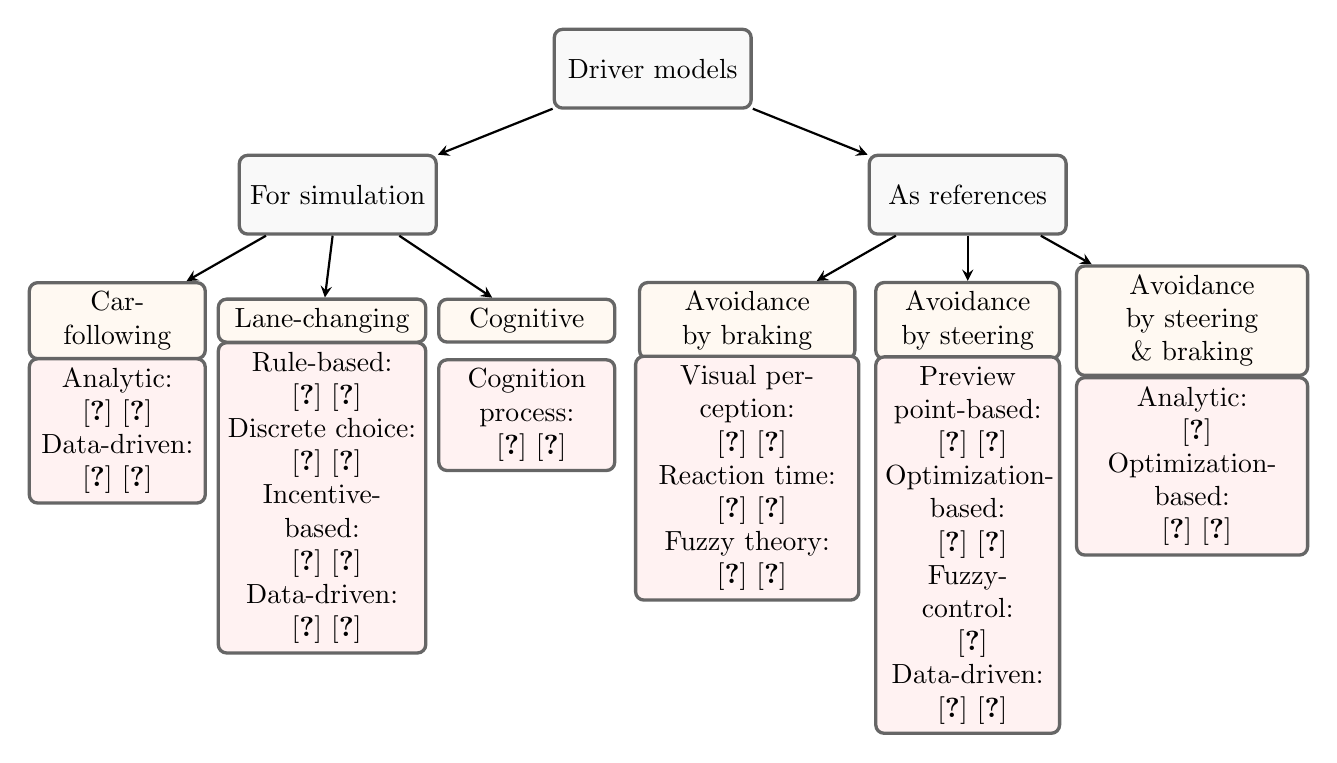
\begin{tikzpicture}[
squared_node/.style={rectangle, draw=black!60, fill=gray!5, rounded corners=3, very thick, minimum width = 2.5cm, minimum height = 1cm},
secondary_node/.style={rectangle, draw=black!60, fill=orange!5, rounded corners=3, very thick, minimum size=5mm},
third_level_node/.style={rectangle, draw=black!60, fill=red!5, rounded corners=3, very thick, minimum size=5mm},
arrow/.style = {thick,->,>=stealth}
]
%Nodes
\node[squared_node]      (root)         {Driver models};
\node[squared_node]      (simulation)       [below of=root, xshift=-4cm, yshift=-0.6cm] {For simulation};
\node[squared_node]      (reference)       [below of=root,xshift=4cm, yshift=-0.6cm] {As references};

\node[secondary_node]    (car-following)       [below of=simulation, xshift=-2.8cm,  yshift=-0.6cm, text width=2.0cm, align=center] {Car-following};
\node[secondary_node]    (lane-changing)       [right of=car-following, xshift=1.6cm, text width=2.4cm, align=center] {Lane-changing};
\node[secondary_node]    (cognitive)       [right of=lane-changing, xshift=1.6cm, text width=2.0cm, align=center] {Cognitive};
\node[secondary_node]    (avoidance by steering)       [below of=reference,  yshift=-0.6cm, text width=2.1cm, align=center] {Avoidance by steering};
\node[secondary_node]    (avoidance by braking) [left of=avoidance by steering, xshift=-1.8cm, text width=2.5cm, align=center] {Avoidance by braking};
\node[secondary_node]    (avoidance by steering and braking)       [right of=avoidance by steering, xshift=1.85cm, text width=2.7cm, align=center] {Avoidance by steering \& braking};

\node[third_level_node]    (cf-Rule-based)       [below of=car-following, yshift= -0.4cm, text width=2cm, align=center] {Analytic: \cite{treiber_congested_2000} \cite{gipps_behavioural_1981} \\
Data-driven: \cite{jia_development_2001} \cite{xu_development_2007} 
};

\node[third_level_node]    (lc-Rule-based)       [below of=lane-changing, yshift= -1.25cm, text width=2.4cm, align=center] {
Rule-based: \\ 
\cite{gipps_model_1986} \cite{yang_microscopic_1996} \\
Discrete choice: \\
\cite{ahmed_models_1996} \cite{toledo_modeling_2003}\\
Incentive-based: \\
\cite{kesting_general_2007} \cite{schakel_integrated_2012}\\
Data-driven: \\
\cite{xie_data-driven_2019} \cite{wang_reinforcement_2018}
};

\node[third_level_node]    (cognitive-based)       [below of=cognitive, yshift= -0.2cm, text width=2.0cm, align=center] {
Cognition process: \\ 
\cite{fries_driver_2022} \cite{siebke_report_2021} \\
};

\node[third_level_node]    (b-braking-based)       [below of=avoidance by braking, text width=2.6cm, yshift=-1.0cm, align=center] {Visual perception: \\
\cite{warren_dynamics_2006} \cite{fajen_calibration_2005}\\
Reaction time: \\
\cite{un_ece_regulation_2021} \cite{shalev-shwartz_formal_2017} \\
Fuzzy theory: \\
\cite{rizianiza_automatic_2021} \cite{mattas_driver_2022}
};

\node[third_level_node]    (b-steering-based)       [below of=avoidance by steering, text width=2.1cm, yshift=-1.85cm, align=center] {Preview point-based: \\
\cite{renski_identification_2001} \cite{sharp_mathematical_2000}\\
Optimization-based: \\
\cite{macadam_application_1981} \cite{macadam_understanding_2003}  \\
Fuzzy-control: \\
\cite{llorca_autonomous_2011} \\
Data-driven: \\
\cite{guo_modeling_2022}  \cite{das_machine_2022}
};

\node[third_level_node]    (braking-steering-based)       [below of=avoidance by steering and braking, text width=2.7cm, yshift=-0.85cm, align=center] {
Analytic: \\
\cite{jurecki_driver_2009}\\
Optimization-based: \\
\cite{falcone_model_2007} \cite{li_emergency_2022} \\
};

%Lines
\draw [arrow] (root) -- (simulation);
\draw [arrow] (root) -- (reference);
\draw [arrow] (simulation) -- (car-following);
\draw [arrow] (simulation) -- (lane-changing);
\draw [arrow] (simulation) -- (cognitive);
\draw [arrow] (reference) -- (avoidance by braking);
\draw [arrow] (reference) -- (avoidance by steering);
\draw [arrow] (reference) -- (avoidance by steering and braking);
\end{tikzpicture}
\caption {\label{fig:Architecture} The review scope of the paper and the classification of driver models. Car-following, lane-changing and cognitive models are discussed in terms of theirs applications in testing AVs in simulations. For driver models as references, braking, steering and a combination of both for collision avoidance are elaborated.} 
\end{figure*}

%...

\section{Driver models for simulations} \label{Driver models for simulations}
In this section, we present a detailed elaboration of driver models for simulation-based testing, including predictive and cognitive models. In particular, car-following and lane-changing models are distinguished in predictive models. Subsequently, an overview of simulation tools with corresponding integrated driver models is given to show their application in AV safety assessment. 

\subsection{Car-following models}
Car-following (CF) is one of the typical behaviors when modeling predictive models. For instance, a car-following model is necessary when testing the adaptive cruise capability of an AV. The model represents the interaction between preceding and following vehicles in the same lane and belongs to microscopic driving behavior models. We divided CF models into analytic and data-driven models according to different modeling methods. 

\textit{Analytic models:} Analytical models provide a physical description of CF models that are constructed based on artificially designed desired destinations and can be used to match real traffic flow. It can be further subdivided into mechanical models, psycho-physical models, cellular automata (CA) models, and adaptable models, as described in \cref{fig:CF_model}. The Gazis-Herman-Rothery (GHR) model, the earliest mechanical model proposed by Chandler et al. \cite{chandler_traffic_1958}, utilizes the relative speed between the preceding and following vehicles as a stimulus item and considers the speed of the preceding vehicle and the time headway as influencing factors of the sensitivity coefficient. The model is expressed by:
\begin{equation} \label{The GHR model}
a_{n}(t+T)=\frac{\lambda v_{n}^{m}(t+T)}{\left[x_{n-1}(t)-x_{n}(t)\right]^{l}}\left[v_{n-1}(t)-v_{n}(t)\right]
\end{equation}
where $n$ refers to the following vehicle; $n-1$ refers to the preceding vehicle; $a_{n}(t+T)$ is the acceleration of the following vehicle at the time $t+T$; $x_{n}(t)$ and $v_{n}(t)$ are the position and velocity of the following vehicle at the time $t$, respectively; $\lambda$ is the sensitivity coefficient; $T$ is the reaction time; $m$, $l$ are coefficients to be calibrated.

Based on the GHR model, several important CF models, such as Gipps model\cite{gipps_behavioural_1981}, Helly model\cite{helly_simulation_1959}, Newell model\cite{newell_simplified_2002}, Intelligent Driver Model (IDM) model\cite{treiber_congested_2000} and Optimal Velocity (OV) model\cite{bando_dynamical_1995}, are successively developed. However, these models often rely on strong assumptions, which could limit their validity. Studies have shown that CF behavior is not purely mechanical but involves the driver's perception, information processing, and decision-making processes\cite{boer_car_1999}. To improve the mechanical models, especially the GHR model, some studies added a memory function\cite{lee_generalization_1966} and the physical state of multiple vehicles ahead\cite{ahmed_modeling_1999} as stimuli to better simulate the CF behaviors of drivers in the real world. 
 
 Inspired by these improved methods, some researchers established psychological-physical models that directly incorporate the driver's perception process. For instance, Wiedemann introduced the term "perceptual threshold" to define the minimum value of a stimulus that the driver can perceive and respond to \cite{wiedemann_simulation_1974}. The basic idea of the model is that once the following driver believes that the relative distance to the preceding vehicle is less than the psychological safety distance, the driver starts to slow down; Because the driver cannot accurately estimate the speed of the preceding vehicle, the following vehicle's speed will be lower than the preceding vehicle's speed for a period of time until the distance between the two vehicles reaches another psychological safety distance. Afterward, the following driver starts to slowly accelerate. Consequently, a repetitive pattern of deceleration, acceleration, and re-acceleration is established. Considering the way the brain estimates the collision time, Andersen et al. \cite{andersen_optical_2007} proposed the Driving-by-Visual-Angle (DVA) model, which uses the visual angle and its change rate as variables for the driver to make acceleration decisions. This model offers a more realistic representation of a driver's reaction while driving. The driving simulator studies show that this model can better fit the driving data.

 However, it is difficult for psychological-physical models to find a balance between the simplicity of the model and the performance due to the complex perceptual processes of the drivers. Cellular Automaton (CA) is considered a promising approach to address this challenge. It is defined as a dynamical system that evolves in discrete time dimensions according to certain local rules in a cellular space that is composed of cells with discrete and finite states. As a result, the discrete-continuous-discrete approximation process can be avoided by applying CA theory to model CF behavior. Since the model developed by Nagel and Schreckenberg (NaSch) \cite{nagel_cellular_1992}, more CA-related driver models are proposed \cite{knospe_towards_2000}\cite{kerner_cellular_2002}\cite{helbing_cellular_1999}.

 Despite being widely used in traffic flow simulation, the CA model falls short of meeting the accuracy required by vehicle simulation. This is due to the contradiction between simplicity and authenticity inherent in the CA algorithm. Therefore, most automotive simulation software still uses mechanical CF models or "psycho-physical" models. Recently, adaptable driver models incorporating driver characteristics are studied. Chen \cite{chen_investigating_2020} investigated intrinsic long-term driving characteristics and their short-term changes using drivers experiencing external stimuli, and proposed a long and short-term driving (LSTD) model that incorporates these changes into the CF model. Long-term driving characteristics were extracted through cluster analysis, and changes after external stimuli were  measured as indicators of short-term driving characteristics. The model was justified using the NGSIM dataset \cite{us_department_of_transportation_next_2016}. Unlike Chen, Liao \cite{liao_car-following_2019} proposed different theoretical models for three traffic states, considering that drivers have varying driving styles in different traffic conditions. Afterwards, numerical tests were conducted to verify the safety, stability, comfort, fuel economy, and consistency of these models with various driving styles in various scenarios.
\begin{figure}[t]
\includegraphics[width=0.42\textwidth]{photo/CFClassification.png}
\centering
  \caption {\label{fig:CF_model} The classification of analytic models. Mechanical Models: A mechanical model is constructed using mathematical and physical equations with a theoretical basis abstracted from traffic phenomena or driving processes. Psycho-Physical Models: A psycho-physical model is constructed based on a driver's perception and response. Cellular Automaton Models: A CA-based model, characterized by discrete time, space, and state variables with localized spatial interaction and temporal causality, has the capability to simulate the spatial-temporal evolution process of complex systems. Adaptive Driver Models: These models consider driver characteristics in order to increase model generalization.} 
\end{figure}

\textit{Data-driven:} With the advent of the era of big data and the rapid improvement of data collection technology, high-precision and large-sample trajectory data can be obtained easily, which stimulates the development of data-driven CF models. Instead of adhering to various theoretical assumptions and pursuing mathematical derivations in a strict sense, data-driven models use non-parametric methods to mine the intrinsic information of trajectory data and build CF models with high prediction accuracy.

By learning from data, artificial neural network methods aim to establish a general description of driving behavior, and they typically have high prediction accuracy in previously observed situations. Therefore, a number of studies utilize artificial neural networks to model CF behavior. For instance, back propagation (BP) neural networks\cite{jia_development_2001}, radial basis function neural network \cite{xu_development_2007} \cite{zhou_application_2009}, and fuzzy neural networks \cite{huang_use_1999} \cite{ma_neural-fuzzy_2006} \cite{li_research_2007} have been continuously applied to model CF behavior. However, the generalization of these models is usually limited.

 Support vector regression is a regression algorithm based on the support vector machine framework. It can be used for regression fitting of trajectory data. This method follows the principle of structural risk minimization and theoretically has stronger data learning and generalization abilities than artificial neural networks. An exemplary application is the model studied by Zhang et al. \cite{zhang_study_2018}. Based on the assumption that drivers tend to exhibit similar driving behaviors when facing the same driving scenario, He et al. \cite{he_simple_2015} searched the \textit{K} similar historical driving scenarios for the most likely driving behaviors, which were then used as model output to generate a KNN (\textit{K}-nearest-neighbor) CF model. Compared to other data-driven models with opaque structures, the KNN model has a clearer modeling structure and is more understandable.

 Deep learning (DL) models, compared to traditional neural network models, usually have multiple hidden layers and a correspondingly huge number of neuronal connection weights, thresholds, and other parameters. Various DL-based CF models have been concentrated in the past five years \cite{zhou_recurrent_2017} \cite{wang_capturing_2018} \cite{liu_learning-based_2022} \cite{lee_integrated_2019}. For instance, both Zhou et al. \cite{zhou_recurrent_2017} and Wang et al. \cite{wang_capturing_2018} proposed CF models based on recurrent neural networks (RNN) by taking continuous historical time series and vehicle dynamic data as input, while the output is the desired speed for the subject vehicle. The results show that their models performs well in predicting the trajectory of the following vehicle. 

However, the high accuracy of DL models comes at the expense of data dependency, high computational costs, and poor generalization. Deep Reinforcement Learning (DRL) has addressed these issues to some extent. Zhu et al.\cite{zhu_human-like_2018} used the difference between simulated speed and observed speed as the reward function and considered a 1 s reaction delay to build a CF model. The model was able to reproduce human-like CF behavior and showed better generalization ability, as the agent learned decision-making mechanisms from the training data, rather than parameter estimation through data fitting. As an extension, Hart et al. \cite{hart_formulation_2021} incorporated the idea of driving styles in the reward function to simulate different driver characteristics.

As the preceding description indicates, CF behavior modeling is actually a challenging task if factors such as accuracy, generalization, computational cost, and driver characteristics are considered. Depending on the specific task, some aspects have to be sacrificed. Additionally, data-driven approaches are intensively studied recently due to their generally high accuracy. 

\subsection{Lane-changing models}
Lane-changing (LC) models usually incorporate three levels while responding to the surrounding environment, as shown in \cref{fig: LaneChallenging}. They are strategic, tactical, and operational levels, respectively. 
\begin{enumerate}
  \item {\bf strategic level} the driver knows about the route in a network, which influences the lane choice, for example, with regard to lane blockages, on-ramps, off-ramps, or other mandatory merges;
  \item {\bf tactical level} maneuvers are selected to achieve short-term objectives such as a decision to pass a slow-moving vehicle or maintain the desired speed;
  \item {\bf operational level} drivers decide about the maneuvers to control their vehicles and determine whether an immediate lane change is both safe and desirable.
\end{enumerate}
\begin{figure}[t] 
\includegraphics[width=0.37\textwidth]{photo/LaneChangeArchitecture.pdf}
\centering
\caption {\label{fig: LaneChallenging} The process of a lane-changing maneuver and its three-level hierarchical division. The desire to reach a goal (strategic level) or increase efficiency (tactical level) motivates lane-changing in decision-making. The gap-selection is responsible for finding a suitable timing. When the timing is right, lane-changing is performed (operational level). } 
\end{figure}

Lane-changing is divided into two types: mandatory lane-changing (MLC) and discretionary lane-changing (DLC) \cite{yang_microscopic_1996} \cite{toledo_modeling_2003} based on driving scenarios. MLC happens when the driver must leave the current lane (e.g., to use an off-ramp or avoid a lane blockage), and DLC happens when the driver performs a lane change to improve driving conditions (e.g., to increase the desired speed in the case of a slow leading vehicle). From the perspective of interaction, free, cooperative, and forced lane-changing are proposed \cite{hidas_modelling_2002} \cite{hidas_modelling_2005}. In cooperative and forced lane-changing, the follower slows down either reluctantly or willingly to create enough space for the lane changer to insert.

\textit{Rule-based:}
The Gipps model \cite{gipps_model_1986} is a type of rule-based LC model. In this model, LC is decided by considering the necessity, desirability, and safety. Factors that affect LC are predefined and their importance is evaluated in a deterministic manner. Three zones depending on the distance to the intended turn are defined to govern the driver's behavior for intended LC. More specifically, a desired speed is kept if the intended turn is far away, while lane changes to the turning lanes or adjacent lanes are considered in the middle zone. When the intended turn is close, the driver focuses on keeping the correct lane and ignores gaining other advantages. Due to the clearly structured triggering conditions, the model has been applied in several traffic simulations. However, the variability in individual driver behavior \cite{rahman_review_2013}, parameter estimation \cite{toledo_modeling_2003}, and applicability in congested scenarios \cite{moridpour_lane_2010} are not addressed.

Yang and Koutsopoulos \cite{yang_microscopic_1996} refined the LC into MLC and DLC, and defined four steps to model a LC maneuver: the decision to consider a LC, choice of the target lane, search for an acceptable gap, and execution of the change, as illustrated in \cref{fig: LaneChallenging}. Different from the Gipps model, the initiation of an MLC is described with a probability that depends on the distance to the intended turn. Although driver behavior variability is modeled to some degree, parameter estimation and validation of the model are missing. To increase the interaction between vehicles during LC, Hidas \cite{hidas_modelling_2002} \cite{hidas_modelling_2005} considered free, cooperative, and forced lane-changing in his model. In cooperative LC, a certain deceleration, determined by the aggressiveness parameter and the urgency of LC, is adopted by the lag driver. The lag gap at the end of deceleration can be obtained based on kinematic equations and compared with the minimum acceptable lag gap to determine if cooperative LC is feasible. Forced LC utilizes the same process as cooperative LC. The differences lie only in the adjusted value of the deceleration of the lagging vehicle and the speed decrease of the subject vehicle.

\textit{Discrete choice-based:} 
In discrete choice-based models, LC decisions are described in a probabilistic manner. Ahmed's model \cite{ahmed_models_1996} \cite{ ahmed_modeling_1999} is representative of this category. He modeled a LC maneuver as a sequence of three steps: the decision to consider LC, the choice of the target lane, and the determination of a sufficient gap. To consider the unusual LC maneuver in congested traffic scenarios where the subject vehicle forces the lag vehicle to yield, he took force merging into account in addition to MLC and DLC. The probability of each type of LC maneuver is calculated in a discrete choice framework. Additionally, whether a gap is accepted or not for MLC, DLC, and forced merging has probability characteristics as well. Consequently, the differences between MLC, DLC, and forced merging are captured in his model. However, a rigid separation between MLC and DLC could be unrealistic in some scenarios because once the MLC is activated, other considerations such as DLC are ignored.  

Therefore, Toledo \cite{toledo_modeling_2003} developed an integrated probabilistic LC model in which MLC and DLC can take effect simultaneously. To evaluate the model, a comparison between separate and integrated MLC \& DLC was performed. The results demonstrated the importance of incorporating trade-offs between MLC and DLC into a LC model.

\textit{Incentive-based:} 
The idea of the incentive choice-based models is to unify the anticipated advantages and disadvantages of a prospective LC. Based on this concept, minimizing overall braking induced by lane change (MOBIL) \cite{kesting_general_2007} was proposed. In MOBIL, both the attractiveness of a given lane (i.e., its utility) and the risk associated with lane changes are measured using single-lane accelerations. When a lane change is considered, it is assumed that a driver makes a trade-off between the expected advantage and the disadvantage imposed on other drivers. The advantages are measured by the difference in the accelerations after and before the lane change, while the disadvantages are quantified by the deceleration imposed on the lag vehicle. Additionally, a "politeness factor" was defined to enable LC from purely egoistic to more cooperative driving behavior. The MOBIL model has the advantage of transferring the assessment of the traffic situation to the acceleration function of the car-following model, allowing for a compact and general model formulation with only a few additional parameters. Nevertheless, empirical justification, model calibration, and validation remain unaddressed. 

The LC model with relaxation and synchronization (LMRS) \cite{schakel_integrated_2012} is another example based on the incentive choice framework. Three different incentives including route following, speed gaining, and right keeping are merged into a single desire. By comparing the single desire with three predefined thresholds, no LC, free LC, synchronized LC, and cooperative LC are distinguished. If the threshold of a free LC is exceeded, LC is performed without preparation. If the single desire is greater than the threshold for synchronized LC, the subject vehicle synchronizes its speed with the target lane and prepares for LC. In cooperative LC, the lagging vehicle creates a gap proactively by following the potential lane changer. This can occur when, for example, the subject vehicle turns indicators or shows lateral movement if its LC desire is large. If the decision to LC is initiated, a gap model similar to MOBIL is utilized in LMRS. To calibrate and validate the model, the data from a segment of highways was applied. The results demonstrated the reproduction of reality in terms of lane volume distributions and lane-specific speeds.

\textit{Data-driven:} 
Due to the lack of flexibility under dynamic driving situations and the resulting poor performance, data-driven approaches are motivated by training properly on a large set of sample data. For instance, a neural network \cite{ren_new_2019}, a deep belief network (DBN) \cite{xie_data-driven_2019} and a support vector machine (SVN) \cite{liu_novel_2019} are applied to model LC decisions. Additionally, deep reinforcement learning (DRL) also shows great potential \cite{wang_reinforcement_2018} \cite{shi_driving_2019} \cite{peng_integrated_2022}. Since a LC process incorporates a sequence of actions and the action to be executed affects the ultimate goal of the task, RL shows great potential to deal with this kind of problem. However, the mapping from state-action pairs to the total return (usually called Q-value) increases significantly with the size of state-action spaces, thus neural networks are applied to model this mapping. 

\subsection{Cognitive models}
The goal of cognitive models is to simulate the human cognition process while driving, which includes perception, recognition, judgment, and operation. Original cognitive models such as ACT-R \cite{anderson_integrated_2004}, Soar \cite{aasman_modelling_1995} and QN-MHP \cite{liu_queueing_2006} are based on psychological cognitive architectures. These models can facilitate the understanding of driver behavior in the context of general human abilities and constraints. However, they are not suitable for simulation in arbitrary dynamic environments due to their complex structures.  

Recently, cognitive models aiming to simulate realistic traffic environments have been proposed. Driver failures that cause crashes can be simulated by taking into account inattentive or distracted driving during the information acquisition process in the cognitive models. A multi-agent traffic simulation software named Re:sim is proposed in \cite{kitajima_nationwide_2022} to model driver agents and their interactions with AVs. In the model, a driver agent perceives the surrounding objects that exist in his line of sight and field of view. The relative states of the observed objects are then calculated, and recognition labels such as preceding or oncoming are assigned to them. Subsequently, hazardous objects are identified, and the risk of collision is estimated. Based on this judgment, the agent decides to operate and react using driving models such as the Weidemann following model.

Similarly, the stochastic cognitive model (SCM) \cite{fries_driver_2022} \cite{witt_modelling_2018} consists of six modules: information acquisition, mental model, situation manager, action manager, action implementation, and driver characteristics. In information acquisition, the visual perception of the driver for perceiving the environment, such as the gaze allocation and fixation duration on a specific area of interest, is modeled. The mental model calculates and stores relevant driving states of observed objects. The situational risk is evaluated by the situation manager, which controls the action manager to provide an appropriate action for the action implementation. Importantly, the SCM model provides the opportunity to parameterize the driver characteristics so that the driver's perception and cognition, compliance with traffic rules can be flexibly adjusted. Unlike the SCM model, the DReaM model \cite{siebke_report_2021} focuses on urban traffic, particularly junction scenarios. Aside from that, the DReaM model has a similar structure to the SCM model. 

\subsection{Simulation tools}
Due to the utility of driver models, some of them are widely used in traffic simulation software, such as in SUMO \cite{behrisch_sumosimulation_2011}, PELOPS \cite{christen_driver_2008}, and Aimsun \cite{casas_traffic_2010}. Table \ref{tab:tableI} summarizes the traffic simulation software with known driver models. We can find that various CF models are utilized in different traffic simulation software, whereas the Gipps \cite{gipps_model_1986} lane-changing model is more frequently integrated into traffic simulation than other LC models. Some recently proposed cognitive models continue to use common driver models where more effort is spent on information acquisition and processing.  

% begin of the table summarizing simulation tools

\begin{table}[!ht]
\caption {\label{tab:tableI} Overview of traffic simulation software with corresponding integrated driver models} 
\begin{tabularx}{\linewidth}{X X X}
% Note: 0.73+0.85+1.09+1.09+1.24 = 5 = # of X-type columns
\toprule
Software & 
\makecell[l]{Car-following \\ models} & 
\makecell[l]{Lane-changing \\ models} \\ 
\midrule
   \rowcolor{Lightgray}
   SUMO \cite{behrisch_sumosimulation_2011} & Kraus \cite{kraus_microscopic_1998} & Krajzewicz \cite{krajzewicz_kombination_2009} \\   
   PELOPS \cite{christen_driver_2008} & Wiedemann \cite{wiedemann_simulation_1974} & \makecell[l]{Sparmann \cite{sparmann_spurwechselvorgange_1978} \\ Gipps \cite{gipps_model_1986} }\\
   \rowcolor{Lightgray}
   PARAMICS \cite{sykes_traffic_2010} & Fritsche \cite{fritzsche_model_1994} & Fritsche \cite{fritzsche_model_1994} \\ 
   MITSIMLab \cite{ben-akiva_traffic_2010} & \makecell[l]{Ahmed \cite{ahmed_modeling_1999} \\ Gazis et al. \cite{gazis_nonlinear_1961} \\ Toledo \cite{toledo_modeling_2003} } & Gipps \cite{gipps_model_1986} \\
   \rowcolor{Lightgray}
   Aimsun \cite{casas_traffic_2010} & Gipps \cite{gipps_behavioural_1981} & Gipps \cite{gipps_model_1986} \\
   SimTraffic \cite{husch_synchro_2006} & Headway-based & Gipps \cite{gipps_model_1986} \\
   \rowcolor{Lightgray}
   VISSIM \cite{fellendorf_microscopic_2010} & Wiedemann \cite{wiedemann_simulation_1974} & Sparmann \cite{sparmann_spurwechselvorgange_1978} \\
   CORSIM \cite{halati_corsim-corridor_1997} & Headway-based & Rule-based \\
   \rowcolor{Lightgray}
   Re:sim \cite{misakidesign_resim_nodate} & Wiedemann \cite{wiedemann_simulation_1974} & Not applicable \\
   \makecell[l]{DReaM \cite{siebke_report_2021} \\ (OpenPASS \cite{dobberstein_eclipse_2017}) } & IDM \cite{treiber_congested_2000} &  Rule-based \\
\bottomrule
\end{tabularx}
\begin{tablenotes}    
    \footnotesize               
    \item CORSIM and DReaM have their own rule-based lane-changing models. Re:sim currently only includes a car-following model.    
\end{tablenotes}  
\end{table}

% end of the table summarizing simulation tools


\section{Driver models as references} \label{Driver models as references}
Driver models used as references for AV safety verification should accurately represent human drivers' driving abilities. Such driving abilities are typically shown in critical scenarios. To describe drivers' driving abilities, the concept of careful and competent driver models is proposed in \cite{un_ece_regulation_2021}. To present a clear scope, the definition of careful and competent is necessary. In the paper, \textit{careful} infers that a driver is capable of identifying a risk in time to avoid unnecessary intense response to a situation, whereas \textit{Competent} means that a driver uses all possible maneuvers to avoid or mitigate a collision.

Thus, we discuss in the following how to identify situation risks in order to trigger which type of driver models. Braking is the most common reaction of drivers in critical situations. However, research \cite{eidehall_toward_2007} shows that if a collision can not be avoided by braking only, steering behavior is also performed by drivers. The combination of braking and steering has the potential to further reduce the probability of a collision. Therefore, all these three types of collision avoidance maneuvers are studied to present a holistic overview of driver models in critical situations. Cognitive models are not discussed even though some of them such as SCM \cite{fries_driver_2022} are supposed to be applicable in critical situations, their validity is not demonstrated. 

\subsection{Braking models} 
\begin{itemize}
  \item \textbf{RQ B1}: \textit{What conditions cause an emergency braking maneuver to be activated?} 
  \item \textbf{RQ B2}: \textit{What models are appropriate for describing emergency braking maneuvers?} 
\end{itemize} 

Regarding the triggering strategy \textbf{RQ B1}:
visual perception and critical metrics are usually used. Visual looming is a typical representative of visual perception, which refers to the optical size and expansion of a preceding vehicle on the retina  \cite{fajen_calibration_2005} \cite{markkula_farewell_2016}. To quantify this visual looming, the inverse tau \cite{lee_theory_1976}, defined as $\tau^{-1}= \dot{\theta} / \theta$, is applied, where $\dot{\theta}$ represents the preceding vehicle's optical expansion rate on the driver's retina, and $\theta$ is the optical size. The inverse tau increases with the collision risk level. However, Markkula \cite{markkula_modeling_2014} argued that a driver's braking is not initiated by exceeding a perceptual threshold, but by the accumulation of noisy perceptual evidence over time. Following this idea, Svärd et al. \cite{svard_computational_2021} proposed a driver model for initiation and modulation of pre-crash brake response to deal with off-road glance behavior. In this model, the initiation time is obtained by the noisy accumulation of perceptual evidence for and against braking.

Besides visual perception, criticality metrics are employed to estimate situation risk. In \cite{un_ece_regulation_2021}, hard braking is applied when a challenging vehicle cuts in and the Time-to-collision (TTC) is smaller than 2 s. According to the study in \cite{schneemann_analyzing_2016}, the TTC for braking onset in urban environments is between 3 and 4 s, while the threshold for participants in the driving test is 2.5 s. Besides TTC, time-to-brake (TTB) is also used in some cases. For instance, a value of 0 is used as the threshold to activate the emergency braking maneuver in \cite{keller_active_2011}. Some driver models aim to model risk without an explicit threshold. Depending on the risk level, different deceleration values are applied. The fuzzy safety model (FSM) \cite{mattas_fuzzy_2020} models the longitudinal risk by defining a safe and an unsafe distance. If the actual distance is larger than the safe distance, no risk exists. Conversely, the highest risk is shown if the actual distance is below the unsafe distance. The risk is interpolated if the distance is between the two distance boundaries. Similarly, the risk-response driver model \cite{zhao_how_2020} utilizes risk field theory to model situation risk and then response correspondingly according to the risk level. 

For emergency braking model \textbf{RQ B2}:
Although existing CF models include deceleration behavior, they are less suitable for use as a comparison reference for AV safety verification because they do not focus on a driver's braking reaction process to imminent situations, but rather on kinematic behavior at the vehicle level, without taking specific driver execution behavior into account. The study in \cite{markkula_review_2012} shows that the Gipps and GHR models exhibit unsatisfying behavior in critical scenarios. Depending on the modeling method, emergency braking models to answer \textbf{RQ B2} can be roughly divided into four categories: visual perception models, reaction time models, and fuzzy theory models.

\textit{Visual perception models:} 
Warren \cite{warren_dynamics_2006} described the braking process based on the tau theory, where the brake-pedal position $z$ should be adjusted according to \cref{eq:TauModel}. $b_\mathrm{pedal}$ is a stiffness parameter determining the speed of pedal adjustments. $\varepsilon$ is the noisy term. $\dot \tau_m$ is the target margin value and $\dot \tau$ is the change rate of $\tau$.
\begin{equation} \label{eq:TauModel}
\Delta z = b_\mathrm{pedal}(\dot \tau_m - \dot \tau) + \varepsilon
\end{equation}
Similar to the $\tau$ model, the deceleration-error model \cite{fajen_calibration_2005} adjusts the deceleration by comparing the current deceleration to an ideal deceleration, where the idea deceleration is defined as the deceleration when $\dot \tau$ equals -0.5. To capture the flexibility of the stiffness parameter in the deceleration-error model, an action boundary for describing the braking urgency is defined in \cite{harrison_affordance-based_2016}, beyond which a collision is unavoidable. If a situation becomes urgent, the proximity to the action boundary decreases, and the driver should apply braking with increasing strength.


\textit{Reaction time models:} 
These models are designed to simulate the response delay that divers may experience during emergency braking. The Japanese driver model proposed in \cite{experts_of_japan_competent_2020} is a typical one in this category, where only braking is considered for collision avoidance. The driver model is separated into the three segments: "Perception", "Decision" and "Braking". A risk perception point is defined to activate the decision and braking. In cut-in scenarios, the risk begins when the cut-in vehicle exceeds the normal lateral wandering zone and the TTC is below 2 s. When the lateral and longitudinal risk are identified, a driver starts to react. The gas pedal is released and the braking pedal is about to take effect, this reaction delay time is 0.75 s. The deceleration rate then increases linearly until to max deceleration 0.744 g. Subsequently, the maximum deceleration rate is maintained. 

Meantime, the Reg157 model is defined in \cite{un_ece_regulation_2021}. This model utilizes TTC to estimate situation risk and apply braking maneuver to avoid collisions. The maximum deceleration is assumed to be at least 6$\mathrm{~m} / \mathrm{s}^{2}$, and the perception time, together with the time needed to achieve the maximum deceleration, is equal to 0.35 s. 

The Responsibility Sensitive Safety model (RSS)\cite{shalev-shwartz_formal_2017} describes the rules that an AV should follow in order to not cause accidents proactively. The longitudinal safety distance, considers the worst situation where the preceding vehicle decelerates with maximum deceleration, and the following vehicle accelerates with maximum acceleration and then decelerates moderately after the reaction time. A conservative distance is obviously assumed from this definition. The RSS model provides safety requirements for a driving strategy. Consequently, it can be used as a reference model to determine the safety responsibility boundary for AVs.

Since the driver reaction time is an important parameter in this type of model and varies among drivers and situations, a classification is made based on the characteristics of reaction time: fixed reaction time \cite{bando_analysis_1998} \cite{treiber_delays_2006}, variable buffer-based reaction time \cite{basak_modeling_2013} \cite{witt_modelling_2018} and random sampling reaction time \cite{przybyla_simplified_2012}. Fixed reaction time means that the reaction time is a fixed value. Variable buffer-based reaction time enables the selection of different independent variables (e.g., speed, distance, or indicator state). For each selected variable, a reaction time is drawn based on the underlying distribution. The random sampling of brake reaction time attempts to model distraction by using sufficient statistical samples to characterize stochastic distributions of reaction time, which can be fed into the microscopic-level CF model for crash prediction \cite{przybyla_simplified_2012}. Despite its simplicity, the reaction time model is assumed to be an important role in critical scenarios, describing the driver's extreme operating behavior in emergency situations. It is an important reference model in AV safety evaluation.

\textit{Fuzzy theory models:}
Fuzzy logic inference systems are known for their great ability to simulate human
reasoning processes as well as the possibility of considering various driving styles and driving environments. Due to these benefits, the development of emergency braking systems using fuzzy logic theory is motivated. Three steps are included in the fuzzy reasoning process. Fuzzification converts the input values to fuzzy values based on predefined rules. Then, the inference engine mimics human reasoning by performing fuzzy inference on the inputs. The output fuzzy variables are finally converted to executable values by defuzzification. The states of the following vehicle and the preceding vehicle are commonly used as input values, and the output values are brake angle or brake pressure \cite{rizianiza_automatic_2021} \cite{basjaruddin_hardware_2016} \cite{mamat_fuzzy_2009}. 
\begin{figure}[!ht]
\includegraphics[width=0.48\textwidth]{photo/ReactionTimeModel.png}
\centering
\caption {\label{fig: ReacitonTimeBraking} An illustration of the braking process for collision avoidance. The situation risk is estimated by a risk perception metric. When an emergency braking maneuver is necessary, deceleration onsets after certain reaction time. The maximum deceleration is either constant or adjusted according to the situation risk level.} 
\end{figure}

Recently, the Fuzzy Safety Model (FSM) \cite{mattas_driver_2022} for rear-end collisions is proposed. Depending on the scenario type, longitudinal and eventually lateral distances are checked against the safe distance to judge if the braking should be initiated. Unlike previous studies, two fuzzy surrogate safety metrics are explicitly employed to evaluate the situation risk. Subsequently, a proper deceleration corresponding to the risk level is performed according to \cref{eq:FSM}.
\begin{equation} \label{eq:FSM}
    D =     
    \begin{cases}
      CFS(D_\mathrm{max} - D_\mathrm{comf}) + D_\mathrm{comf} & \text{if $CFS > 0$}\\
      PFS \cdot D_\mathrm{comf} & \text{if $CFS = 0$}\\
    \end{cases} 
\end{equation}
where the Proactive Fuzzy surrogate Safety metric (PFS) and the Critical Fuzzy surrogate Safety metric (CFS) are the two metrics to evaluate situation risk. $D_\mathrm{max}$ and $D_\mathrm{comf}$ represent the maximum and comfortable deceleration of the following vehicle.

From the above analysis, we discover the following commonalities of the discussed collision avoidance braking models. First, a risk perception metric is essential in order to trigger the braking model. Either visual perception or criticality metrics are applied to estimate the situation risk. Second, most works consider the reaction parameter either explicitly (reaction time models) or implicitly (fuzzy theory models) in their models. Third, the deceleration in some models can be adapted according to the risk level, while it is a fixed profile when the model is triggered. As a result, we use \cref{fig: ReacitonTimeBraking} to summarize the braking models. Due to the special application for AV safety verification, interpretability is an important factor for the models in order to provide an understandable reference for such safety-critical systems. Additionally, near-crash and crash data are limited, which further hinders the application of data-driven models in this case.

\begin{figure}[!ht]
  \begin{minipage}[t]{0.95\linewidth}
    \includegraphics[width=\linewidth]{photo/steering1.png}%
  \end{minipage}\hfil
  
  \begin{minipage}[t]{0.95\linewidth}
    \includegraphics[width=\linewidth]{photo/steering2.png}%
  \end{minipage}\hfil
  
  \begin{minipage}[t]{0.95\linewidth}
    \includegraphics[width=\linewidth]{photo/steering3.png}%
  \end{minipage}%
  \caption {\label{fig:steering_model} The illustration of three evasive steering models using the preview method. (a) models using a single preview point; (b) models optimizing over a preview horizon; (c) models using multiple preview points.} 
\end{figure}

\subsection{Evasive steering models}
Similar to the braking models, two research questions should be answered regarding the evasive steering models:
\begin{itemize}
  \item \textbf{RQ S1}: \textit{What conditions cause an evasive steering model to be activated?} 
  \item \textbf{RQ S2}: \textit{What models are appropriate for describing evasive steering maneuvers?} 
\end{itemize}

For the triggering strategy \textbf{RQ S1}:
Depending on the risk level, an evasive steering maneuver should be conducted or not. Despite the simplicity of TTC, it is the most common metric to activate such maneuvers. For instance, A TTC threshold of 2.5 s is utilized in \cite{llorca_autonomous_2011}. They demonstrated that the proposed approach can perform human-like pedestrian collision avoidance maneuvers by steering with a maximum driving speed of 30 km/h. Zhao et al. \cite{zhao_emergency_2019} consider 0.75 s for the threshold of TTC for an emergency evasion maneuver. Similarly, a two-dimensional TTC with a threshold of 5 s is defined for a data-driven evasive steering model \cite{guo_modeling_2022}. In \cite{keller_active_2011}, an evasive maneuver is activated when the Time-to-Steer (TTS) is 0. 

A "threat metric" related to acceleration or jerk level is utilized to trigger an evasion maneuver, which is defined by a cubic polynomial with zero derivatives at the knots. The number of knots and their position depends on the number of objects along the path and their position. However, the trigger threshold is not presented  \cite{eidehall_real_2013}.

Some studies define the trigger moment implicitly. Isermann et al. \cite{isermann_collision-avoidance_2012} argue that the timing to evade is determined by at what distance the evasion must be executed so that a collision is still preventable. They utilize a sigmoid function to describe the evasive trajectory. Park et al. \cite{park_emergency_2021} assume that braking is first applied, and the steering maneuver must wait until collision by braking is no longer possible. Additionally, the expected lateral acceleration should be greater than a threshold under which the collision can be avoided by the driver's steering. 

For the evasive steering model \textbf{RQ S2}: Typically, lateral position and heading angle errors are used to model an evasive steering model. We divide the existing evasive steering model into five categories based on the various ways to calculate the errors: preview point-based, optimization-based, fuzzy-control models, data-driven models. In particular,the models using a single preview point, the models using multiple preview points, and the models using optimization over a preview horizon are illustrated in \cref{fig:steering_model}.

\textit{A single preview point:} 
A preview point is the simplest way to achieve the desired steering angle for an evasive maneuver. Based on the lateral position or heading angle at a future point, the steering angle $\delta(t)$ is obtained \cite{renski_identification_2001}.
\begin{equation}
\delta(t) =  \textit{K} \varepsilon(\textit{t}-T_\text{R})
\end{equation}
where $\varepsilon(t)$ is the angle between the heading of the vehicle and the preview point, $T_R$ is the driver reaction time, and \textit{K} is a gain constant.
As an improvement, Zhao et al. \cite{zhao_emergency_2019} take both lateral distance and heading angle at the preview point into account. Nevertheless, if the preview point is close, the control performance is poor. Conversely, inappropriate action could occur based on solely the preview information at the time of its acquisition. 

\textit{Optimization over a preview horizon:} 
Instead of determining the steering angle based on a single future point, this class of model optimizes the steering angle over a horizon (sequential multiple points). The model proposed by MacAdam \cite{macadam_application_1981} \cite{macadam_understanding_2003} minimizes the predicted lateral deviation from a desired path to determine the steering wheel angle. In this category, motion predictive control (MPC) is usually utilized.

\textit{Multiple preview points:} 
Models optimizing over a preview horizon show good stabilization capabilities in relation to rapid maneuvers. However, the models can be computationally intensive and may not converge if the constraints are not well-defined. To approximate this type of model but achieve the same performance, models using multiple preview points are an alternative. In this case, the driver model \cite{sharp_mathematical_2000} utilizes a weighted sum of current and previewed path deviations $e_i$, and the heading error $e_\psi$ at the current position, as expressed by \cref{eq:multiple preview points}. $\textit{K}_\psi$, $\textit{K}_1$ and $\textit{K}_i$ are model constant parameters, whereas the number $n$ represent the preview points.

\begin{equation} \label{eq:multiple preview points}
\delta = \textit{K}_\psi e_\psi + \textit{K}_1 e_1 + \textit{K}_p \sum_{i=2}^{n} \textit{K}_i e_i
\end{equation}

\textit{Fuzzy-control:} 
In \cite{llorca_autonomous_2011}, a fuzzy controller is applied to perform evasive steering maneuvers. The fuzzy reasoning process incorporates three stages. The lateral displacement and vehicle speed are converted to a fuzzy value in the fuzzification stage. Human-like reasoning process to yield the values of the output fuzzy variables is conducted in the inference engine. In the defuzzification stage, the fuzzy output values are converted to crisp values.

\textit{Data-driven:} 
A deep deterministic policy gradient (DDPG) algorithm \cite{guo_modeling_2022}, which could learn the sequential decision-making process over continuous action spaces, was used to model evasive behaviors. Another data-driven model proposed by Das and Mishra \cite{das_machine_2022} attempted to avoid collisions using left and right turn maneuvers that are learned from a dataset.

\begin{figure}[!ht]
\includegraphics[width=0.5\textwidth]{photo/SteeringAvoidance.png}
\centering
\caption {\label{fig: SteeringIntroduction} The process of an evasive steering maneuver performed by a driver. If a driver perceives a situation risk that necessitates a response, the steering maneuver is executed by minimizing errors to a given evasion path after the reaction time.} 
\end{figure}

\cref{fig: SteeringIntroduction} illustrates the process of the steering maneuver in case of a critical situation. The situation risk is estimated. When the steering maneuver is possible, e.g., enough free space at the steering side, The steering angle is typically determined and executed by minimizing errors to a reference after a certain reaction time.

\subsection{Braking and steering models}
Under rather critical situations or a situation where a collision is unavoidable, simultaneously braking and steering maneuvers are appropriate to mitigate the collision severity as much as possible. The driver model proposed by Jurecki and Stańczyk \cite{jurecki_driver_2009} synthetics these two maneuvers analytically. In the driver model, the braking model is described as:
\begin{equation} \label{eq:SteeringandBraking1}
\textit{D} + \textit{W}_1 \dot{D} = \textit{W}_2\Delta{y}(t - T_\text{R}) + \textit{W}_3 \frac{v_{\text{rel}}}{d_{\text{rel}}}
\end{equation}
where \textit{D} is deceleration; $\Delta{y}$ represents the lateral relative distance; $T_\text{R}$ is the driver's reaction time; $\textit{W}_1$, $\textit{W}_2$ and $\textit{W}_3$ are model constant parameters. $v_{\text{rel}}$ and $d_{\text{rel}}$ are the longitudinal relative velocity and distance, respectively. The corresponding steering model $\delta$ is expressed by:
\begin{equation} \label{eq:SteeringandBraking2}
\delta + \textit{W}_4 \dot{\delta} = \textit{W}_5 \Delta{y} (t - T_\text{R})
\end{equation}
$\textit{W}_4$ and $\textit{W}_5$ are another model parameters. These model parameters are identified based on 450 trials with 30 drivers.

Schorn and Isermann \cite{schorn_automatic_2006} employ a sigmoidal function to generate the desired trajectory, which is followed by a feedforward control to execute braking and steering. Similarly, many studies \cite{falcone_model_2007} \cite{li_emergency_2022} \cite{wang_integrated_2022} \cite{hajiloo_integrated_2021} nowadays use the model predictive control (MPC) technique to control the steering angle and the brakes with a given following path. As a result, the optimization-based methods demonstrate a tendency to deal with simultaneous braking and steering. 

\section{Applicability} \label{Applicability}
In this section, we first define evaluation metrics for driver models in the two applications discussed in the paper. Next, we summarize and categorize the aforementioned driver models based on their model characteristics. We then analyze the potential applications and suitability of different driver model categories for the two different applications based on the proposed evaluation metrics to finally answer the \textbf{RQ3}.

\subsection{Evaluation metrics}
A driver model for simulation is primarily used in simulations to evaluate AV safety in mixed-traffic environments with human drivers. Therefore, the driver model shall replicate human driver behavior as closely as possible, including the variability of the behavior itself. To fulfill this evaluation metric, a driver model shall meet four evaluation metrics: variability, adaptability, simplicity, and accuracy. These evaluation metrics are presented in \cref{tab:tableII}, along with their descriptions and examples of typical models that best meet each evaluation metric. Additionally, possible research focus is provided, for which this evaluation metric is particularly relevant.

A driver model as a reference is used as a benchmark to evaluate AV safety performance, and it shall represent the capabilities of careful and competent drivers. Its underlying logic is that an AV shall demonstrate superior performance compared to a careful and competent human driver in critical scenarios, i.e., it can successfully avoid collisions in at least the same critical scenarios in which a careful and comperent human driver can do. Therefore, a benchmark driver model for AV safety evaluation should satisfy four evaluation metrics: representativeness, maneuvers-coverage, interpretability, and accuracy. These evaluation metrics are also listed in \cref{tab:tableII} together with the descriptions, typical driver models and possible research focus.

% begin of the table introducing evaluation metrics

\begin{table*}[!ht]
\caption {\label{tab:tableII} The metrics for evaluating driver models in terms of their applications in AV safety assessment } 
\begin{tabularx}{\linewidth}{p{1.5cm} p{2cm} p{7.5cm} Z Z}
\toprule
Application & 
\makecell[l]{Evaluation metrics} & 
\makecell[l]{Descriptions} & 
\makecell[l]{Typical models} &
\makecell[l]{Possible research} \\ 
\midrule
   \multirow{32}{*}{Simulation} & Variability & The driver model shall reflect the variability in human driver behavior, which arises from the complex processes of perception, cognition, and decision-making. Even for an identical driver in the same situations, various behaviors including errors may be exhibited. Although the likelihood of errors is low, they shall be considered since they can lead to hazardous scenarios for AVs. Therefore, the driver model shall demonstrate variability in simulations and avoid oversimplification or neglect of any behaviors that may be critical for AV safety assurance. & The model with stochastic brake reaction time \cite{przybyla_simplified_2012}, \newline the stochastic cognitive model (SCM) \cite{fries_driver_2022}  & Testing an AV's ability to handle the behavioral diversity of surrounding human drivers within the same scenario. \\ \cline{2-5} 
   & Adaptability & The driver model shall demonstrate its adaptability to different situations. Human driver behavior can vary across different situations. Thus, the driver model needs to be able to adapt to these varying situations and reflect the corresponding changes in driver behavior. This adaptability is essential for accurately modeling human driving behavior and evaluating AV safety performance in simulations. & The model with driver characteristics included \cite{liao_car-following_2019}, \newline the model proposed by Zhang et al.\cite{zhang_study_2018} & Mileage-based simulation \\  \cline{2-5}
   & Simplicity & The driver model shall be designed to have relatively low computational complexity. In order to capture the diverse human driver behavior and different driving situations, simulations must be run on a large number of scenarios or driving miles, often necessitating the use of methods such as the Monte Carlo method. Moreover, concrete scenarios frequently involve multiple vehicles controlled by human drivers. Therefore, reducing the complexity of the driver model can help to minimize computational costs. & GHR model\cite{xie_data-driven_2019}, IDM model \cite{treiber_congested_2000} & Monte-Carlo simulation, Mileage-based simulation, Coverage-oriented simulation \\  \cline{2-5}
   & Accuracy & Accuracy refers to the degree to which a driver model is able to reproduce the actual driving behavior of human drivers. In other words, it measures how closely a model's output matches the real-world data. A highly accurate driver model will produce results that are very close to the actual human driving behavior in different scenarios. This is important for valid and credible AV safety assessment.  & DBN \cite{xie_data-driven_2019}, \newline the model based on a gated RNN network \cite{wang_capturing_2018} & Microscopic simulation \\  \cline{1-5}
   \multirow{18}{*}{Reference} & Representativeness & The driver model shall be representative of the abilities of a careful and competent human driver in critical situations. Representativeness does not mean collision-free, as the model should not be expected to avoid all collisions. Instead, it should match the abilities of a careful and competent human driver in these situations. & The Japanese driver model \cite{un_ece_regulation_2021}, \newline the FSM \cite{mattas_fuzzy_2020} & Addressing the question of “how good is good enough” in AV evaluations. \\ \cline{2-5} 
   & Maneuver-coverage & When faced with danger, humans often weigh several possible collision avoidance maneuvers, including braking, steering, and a combination of both. If a model is limited to only braking maneuvers, it demonstrates only the ability of human drivers under limited conditions because braking is not always the optimal collision avoidance strategy. Therefore, the driver models as references shall include different possible collision avoidance maneuvers. & The driver model proposed by Jurecki et al. \cite{jurecki_driver_2009}, \newline The MPC-based model & Guidance on improving collision avoidance capability of AVs in emergency situations \\  \cline{2-5}
   & Interpretability & Using a driver model as a benchmark for evaluating AV safety performance means that it serves as a criterion in the evaluation. As a criterion, its definition should be clear and interpretable to ensure the reliability of the evaluation and gain the public's trust. & Models using the preview method \cite{renski_identification_2001}, \newline the RSS model \cite{shalev-shwartz_formal_2017} & Defining benchmark for AV safety assessment \\  \cline{2-5}
   & Accuracy & Accuracy refers to the ability of the human driver model to accurately represent the peak performance of human drivers in critical scenarios. The accuracy of the human driver model is critical in ensuring that an AV is evaluated against a realistic and representative benchmark & The FSM \cite{mattas_driver_2022}, \newline the DDPG model \cite{guo_modeling_2022} & Guidance on the design of vehicle dynamics under extreme conditions \\
\bottomrule
\end{tabularx}
\begin{comment}
\end{comment}
\end{table*}

% end of the table summarizing simulation tools

\subsection{Summarization of human driver models}
Regardless of whether they are used for simulation or as a reference, human driver models are commonly developed based on diverse mathematical models. Based on the different abstract mathematical expressions, human driver models can mainly be divided into the following categories:

\textit{Linear model:} This type of model simulates human driver behavior by establishing a linear relationship between the factors considered and the maneuvers taken by human drivers, such as the GHR \cite{xie_data-driven_2019} and IDM \cite{treiber_congested_2000} car-following models.

\textit{Non-linear model:} The perceptual, judgment, and decision-making processes of human drivers are complex and nonlinear. Many researchers choose to improve the complexity of the model and better fit human driver behavior by adding nonlinear terms to the model. Compared to pure data-driven models, the non-linear models in this category have relatively lower complexity or dimensionality. The methods used for nonlinearization mainly include the following categories: 1) \textit{Nonlinearity through activation function:} Nonlinearity is achieved by adding a nonlinear activation function, such as the perceptual threshold introduced in \cite{andersen_optical_2007}  (similar to the ReLU function \cite{agarap_deep_2018}), to the model. 2) \textit{Nonlinearity through integral terms:} Nonlinearization is achieved by adding integral terms to the model, such as the memory function introduced in \cite{ahmed_modeling_1999}. 3) \textit{Nonlinearity through adaptive coefficient:} Nonlinearization of the model is achieved by adaptively adjusting coefficients based on situations, such as the model proposed by Liao et al. \cite{liao_car-following_2019} 4). \textit{Nonlinearity through fuzzy term:} Nonlinearization of the model is achieved by introducing fuzzy items, such as fuzzy logic in \cite{kikuchi_car-following_1992}. 5) \textit{Nonlinearity through stochasticization:} Nonlinearization of the model is achieved by introducing random terms, such as reaction time in \cite{przybyla_simplified_2012}.

\textit{Optimization-based model:} Unlike non-linear models, it is in some cases impossible to model the relationship between influence factors and control variables mathematically. However, it is able to characterize these models by defining objective functions and constraints. According to a given objective function, this model optimizes driving behavior to achieve the optimal result. It incorporates the evasive steering model proposed by MacAdam et al. \cite{macadam_application_1981} \cite{macadam_understanding_2003}, as well as the widely used MPC technique.

\textit{Data-driven model:} Data-driven models capture the complexity of human driver behavior by adopting high-dimensional nonlinear models, such as the recurrent neural network in \cite{zhou_recurrent_2017} and DBN in \cite{xie_data-driven_2019}, and training them with real human driver data. Although there are differences in the degree of reliance on data in the models, data is indispensable. 

\subsection{Applicability analysis}
This subsection evaluates the summarized driver models in terms of their applications for AV safety assessment and verification. Based on the proposed metrics, a comparison of linear, non-linear, optimization-based, and data-driven models is conducted. As a result, the dis- and advantages of each type of driver model are presented, which can guide developers to select proper driver models for their different purposes.  

In the context of simulations, \cref{tab:tableIII} provides a comparison of different categories of driver models in meeting the proposed evaluation metrics. Nonlinear and data-driven models demonstrate superior capability in meeting more evaluation metrics compared to linear and optimization-based models, particularly three out of the four evaluation metrics. The key distinguishing factor between nonlinear and data-driven models is the trade-off between complexity and accuracy. Nonlinear models exhibit relatively lower complexity and are thus more appropriate for scenarios that demand extensive simulation calculations, such as those involving high mileage and multi-scenario coverage. In contrast, data-driven models, particularly those utilizing deep learning techniques, consider more feature dimensions and exhibit higher-order nonlinearity, which leads to higher accuracy but also entails increased complexity and computational costs.

\begin{table}[!ht]
\caption {\label{tab:tableIII} Evaluation and Comparison of Driver Models with Different Model Characteristics in Terms of their suitability for Simulation Purposes} 
\begin{tabularx}{\linewidth}{l X X X X}
\toprule
Evaluation metrics & 
\makecell[l]{Linear} & 
\makecell[l]{Non-linear} &
\makecell[l]{Optimi- \\ zation}& 
\makecell[l]{Data-driven} \\ 
\midrule
    Variability & - & + & - & + \\
    Adaptability & - & + & + & + \\
    Simplicity & + & + & - & - \\
    Accuracy & - & - & - & + \\
\bottomrule
\end{tabularx}
\begin{tablenotes}    
    \footnotesize               
    \item The "+" symbol indicates that the model is able to meet the evaluation metric. Conversely, "-" means the metric is a challenge for the model.
\end{tablenotes}  
\end{table}


In the application where driver models serve as a reference, the comparative results are summarized in \cref{tab:tableIV}. The non-linear model is capable of meeting the evaluation metrics related to emergency braking. On the other hand, the optimization-based model can simultaneously fulfill the evaluation metrics for simulating both braking and steering avoidance behaviors, while demonstrating better interpretability. Conversely, the data-driven model, although able to meet the representativeness, accuracy, and even maneuver-coverage evaluation metrics, is disadvantaged by its lack of interpretability and transparency. As a benchmark for evaluating the performance of AV, interpretability and transparency are crucial for regulation \cite{fagnant_preparing_2015} and insurances \cite{grosso_how_2021}. The clear definition of the cost function, weights, and constraints of the optimization-based model are more easily understood by humans and can be explained to the public. Therefore, when constructing a driver model for reference, the optimization-based model can be a good choice.

\begin{table}[!ht]
\caption {\label{tab:tableIV} Evaluation and Comparison of Driver Models with Different Model Characteristics in Terms of their suitability for Reference Purposes} 
\begin{tabularx}{\linewidth}{l X X X X}
\toprule
Evaluation metrics & 
\makecell[l]{Linear} & 
\makecell[l]{Non-linear} &
\makecell[l]{Optimi- \\ zation}& 
\makecell[l]{Data-driven} \\ 
\midrule
    Representativeness (\textit{B}) & + & + & + & + \\
    Representativeness (\textit{S}) & - & - & + & + \\
    Maneuver-coverage & - & - & + & + \\
    Interpretability & + & + & + & - \\
    Accuracy (\textit{B}) & - & + & + & + \\
    Accuracy (\textit{S}) & - & - & + & + \\
\bottomrule
\end{tabularx}
\begin{tablenotes}    
    \footnotesize               
    \item The "+" symbol indicates that the model is able to meet the evaluation metric. Conversely, "-" means the metric is a challenge for the model. \textit{B}" stands for braking and "\textit{S}" stands for steering. The combination of different driver models is not considered in each category. The data-driven category is supposed to be capable of modeling diverse collision avoidance maneuvers given enough relevant data.
\end{tablenotes}  
\end{table}

\subsection{Careful and competent driver models}
Based on the analysis, we propose an architecture to describe a careful and competent driver model, as illustrated in \cref{fig: idealmodel}. For risk perception, the common used metrics with a fixed threshold is unable to describe the driving behavior reasonably in cases of an emergency situation. In contrast, the fuzzy surrogate safety metrics provide promising results. A corresponding reaction is performed by continuously observing the metrics while driving to avoid sudden or too late operations.

The reaction process of a competent driver includes three stages. The braking maneuver is the first choice. Even though the evasive maneuver is theoretically better than the braking maneuver at high velocities \cite{ackermann_collision_2014}, a study \cite{adarns_review_1994} shows that drivers are more likely to brake in critical situations. if a collision cannot be avoided by the braking maneuver, the evasive maneuver is applied because a shorter distance is required. If a collision is inevitable, simultaneous braking and steering are performed to mitigate the collision severity. The driver models corresponding to these three stages can be chosen according to the aforementioned driver models considering the evaluation metrics.    

\begin{figure}[ht]
\includegraphics[width=0.5\textwidth]{photo/Architecture.png}
\centering
\caption {\label{fig: idealmodel} The architecture of a careful and competent driver model for handling critical scenarios. In stage 1, the braking is applied based on the estimated risk; in stage 2, the steering maneuver is executed if free space on the side exists; in stage 3, simultaneous braking and steering are initiated to mitigate a collision. For each stage, suitable driver models can be selected based on a user's demand using the proposed evaluation metrics.} 
\end{figure}

\section{Discussion} \label{Discussion}
In this paper, we investigated the role of driving models in the safety assessment of AVs. By addressing three research questions, the guidance for safety engineers to select appropriate driving models either for AV safety evaluation in simulations or for determining AV safety performance level compared to careful and competent drivers was provided. Meanwhile, we presented an architecture of a reference driver model for tackling critical scenarios. This architecture portrays the extreme capabilities of a careful and competent human driver and thus can be considered a reference when it comes to AV release. To the authors' best knowledge, this is the first work that summarizes driver models in terms of their applications for AV safety assessment.

For \textbf{RQ1}, we proposed evaluation metrics for driver models when applying them for AV safety assessment. These metrics pose requirements on new developing driver models according to their applications. Additionally, we found that predictive and cognitive models are required in simulation-based testing. More specifically, cognitive models are suitable for large-scale environments where modeling human driving errors is necessary. In contrast, predictive models are the choice when testing AVs in single concrete scenarios. When taking a driver model as a reference for AV safety verification, drivers' peak capability in critical scenarios should be modeled.

For \textbf{RQ2}, we presented an overview of driver models based on the defined scope in the paper. Various car-following and lane-changing models were described under the category of predictive models. It is observed that applying artificial intelligence (AI) to model specific driving behavior shows a trend. Due to the inscrutability of AI, Hybrid models that combine AI and analytic models to increase explainability while maintaining high fidelity are being investigated \cite{bhattacharyya_hybrid_2021}. Additionally, cognitive models that aim to model driving behavior both in normal traffic and critical scenarios show promising results except for the high model complexity. In critical situations, we considered possible maneuvers including collision avoidance by braking, collision avoidance by steering, and collision avoidance by simultaneous braking and steering in order to build a competent driver. The models that correspond to those possible maneuvers are outlined, which can be served as reference models for AV safety verification. In addition, we have always taken the timing for triggering avoidance maneuvers into account, which is beneficial when designing AV functions. Lastly, we provided an architecture to illustrate drivers' extreme driving capability when faced with critical situations, which can be used to build a driver model that poses a higher performance boundary for AV safety verification. 

For \textbf{RQ3}, we first proposed several metrics to assess the driver models that are discussed in the paper. Based on these metrics, we are able to analyze the strengths and weaknesses of each driver model, which facilitates the determination of its applicability. For the driver models for simulation, non-linear and data-driven models are the preferred choices. When choosing between the two, a trade-off needs to be made between complexity and accuracy. If greater accuracy is desired and the additional computational cost of higher complexity is acceptable, a data-driven model may be chosen. Conversely, a non-linear model may be chosen if a relative lower accuracy can be tolerated in exchange for the lower computational cost. As computer hardware performance continues to rapidly advance, the high complexity of data-driven models may no longer be a concern in the future, making them the optimal choice. Regarding driver models as a reference, optimization-based models are the optimal choice since they can exhibit powerful performance in both steering and braking for collision avoidance, and have good interpretability. If the interpretability issue of data-driven models can be addressed in the future, they could also become a good choice.

Compare to the work in \cite{siebke_what_2022}, we analyzed in-depth various driver models as references for AV safety verification and discussed their applicability, while they focus on a discussion about human error modeling in traffic simulations. Additionally, a discussion of a suitable architecture of a reference driver model in their work is missing. For some other surveys, either they only review one category of driver models like car-following models \cite{han_modeling_2022}, or driver models for AV safety assessment are not considered in their reviews \cite{singh_analyzing_2021} \cite{ park_review_2022}. 

Based on the defined scope in \cref{Requirements and scope}, we limit our review to the driver models that are useful either for the safety assessment of AVs in a simulation environment or for AV approval by showing their reference roles. Thus, other topics like driver behavior analysis are not considered. In addition, there may be some selection bias for relevant papers. However, the commonly used driver models are identified carefully. Thus, a significant influence on our summarized results is avoided. The proposed metrics to evaluate different types of driver models are summarized considering our two applications for AV safety assessment. Therefore, they are limited to our purpose, and a comprehensive evaluation of driver models including their applications in other domains should be further studied.    

Generally, our paper provides a fundamental consideration of currently existing driver models for AV safety assessment. On one hand, it can aid policymakers such as the UNECE committee to choose appropriate driver models when drafting regulations for AV approval. On the other hand, safety or simulation engineers could utilize suitable driver models depending on their demands to conduct their simulations in order to provide evidence to support a holistic safety argumentation for their developed AVs.

In summary, the paper conducts a survey about diver models in order to answer three research questions regarding their applications for AV safety assessment. By summarizing the identified relevant papers, we are able to present guidance on what type of driver models are suitable for what type of task. Compared with other related works, our work presents a holistic overview of driver models with a special focus on their applications in AV safety assessment. Though some limitations exist, the survey is generally useful for policymakers and developers. 

\section{Conclusion and future work} \label{Conclusion and future work}
The paper presents a discussion of driver models in terms of their application in AV safety assessment. Based on the results, we have the following findings: 1) cognitive models show a driver model development trend, which aims to be applicable in both normal traffic and critical situations; 2) collision avoidance by steering, and collision avoidance by simultaneous steering and braking are less studied than collision avoidance by braking. The proposed architecture combining three stages of collision avoidance maneuvers is promising for establishing a careful and competent reference model; 3) the interpretability property of driver models is important for safety-critical systems such as AVs.

Meantime, these findings indicate future working directions. More open-sourced driver simulator datasets and crash datasets are desirable in comparison to the number of open-sourced naturalistic driving datasets such as HighD \cite{krajewski_highd_2018} and AD4CHE \cite{zhang_ad4che_2023}. The data is valuable for studying driver steering, steering and braking behavior in critical situations. In this way, a holistic driver model incorporating different maneuvers at different stages of a collision could be created as a reference instead of a single emergency braking model. Explainable AI must be prioritized in order to achieve both high interpretability and performance. In all, the paper provides a solid foundation for future driver models for AV safety assessment.




%{\appendices
%\section*{Proof of the First Zonklar Equation}
%Appendix one text goes here.
% You can choose not to have a title for an appendix if you want by leaving the argument blank
%\section*{Proof of the Second Zonklar Equation}
%Appendix two text goes here.}



\bibliographystyle{IEEEtran}
\bibliography{references}


\newpage

\vfill

\end{document}

% begin of car-following models. RUILIN please complete this figure.


